\documentclass[12pt, letterpaper]{article}
\usepackage{graphicx} % Required for inserting images
\usepackage{hyperref}
\usepackage{listings}
\usepackage{amssymb}
\usepackage{amsmath}
\usepackage[english]{babel}
\usepackage{nicefrac, xfrac}
\usepackage{mathtools}
\newcommand{\acc}{\\\hphantom{}\\}
\usepackage[table,xcdraw]{xcolor}
\usepackage[paper=a4paper,left=20mm,right=20mm,bottom=25mm,top=25mm]{geometry}
\renewcommand{\labelenumii}{\arabic{enumi}.\arabic{enumii}}
    \renewcommand{\labelenumiii}{\arabic{enumi}.\arabic{enumii}.\arabic{enumiii}}
    \renewcommand{\labelenumiv}{\arabic{enumi}.\arabic{enumii}.\arabic{enumiii}.\arabic{enumiv}}
\title{Ristrutturazione Go}
% \author{ Giacomo Biribicchi \and Marco Casu \and Christian Di Manno \and Alessandro Gautieri }
\date{}


\begin{document}

\maketitle


\section{Documenti di Specifica}
\subsection{Tipi di Dato}
\subsubsection{Domini}
\begin{itemize}
    \item create domain $Intger>0$ as integer
    default 0
    check $(value>=0);$
    \item create domain $Komi$ as real
    default 0
    check $(value>=0 and value <=10);$

\end{itemize}
\subsubsection{Tipi}
\begin{itemize}
    \item create type as enum Punteggio $=$ \{b : $Integer>0$, n : $Integer>0$\}
    \item create type as enum Regole = \{'cinese','giapponese'\}
    \item create type as enum Anno = ("19" or "20") concat ["00","99"]\{1\}
    \item create type as enum Giocatore = \{'bianco','nero'\}
\end{itemize}
\section{Vincoli Esterni Ristrutturazione}
\begin{itemize}
    \item $\exists g,b,n,p  Giocatore(g) \land Partita(p) \rightarrow GiocaBianco(g,p) \lnot GiocaNero(g,p)$
    \item $\lnot \exists g,p,ep, er Giocatore(g) \land Partita(p) \land EsitoPunteggio(ep) \land EsitoRinuncia(er) \land$\acc
    $ PartitaEsitoRinuncia(p,er)\rightarrow \lnot PartitaEsitoPunteggio(p,ep)$
\end{itemize}


\section{UML}
\begin{center}
    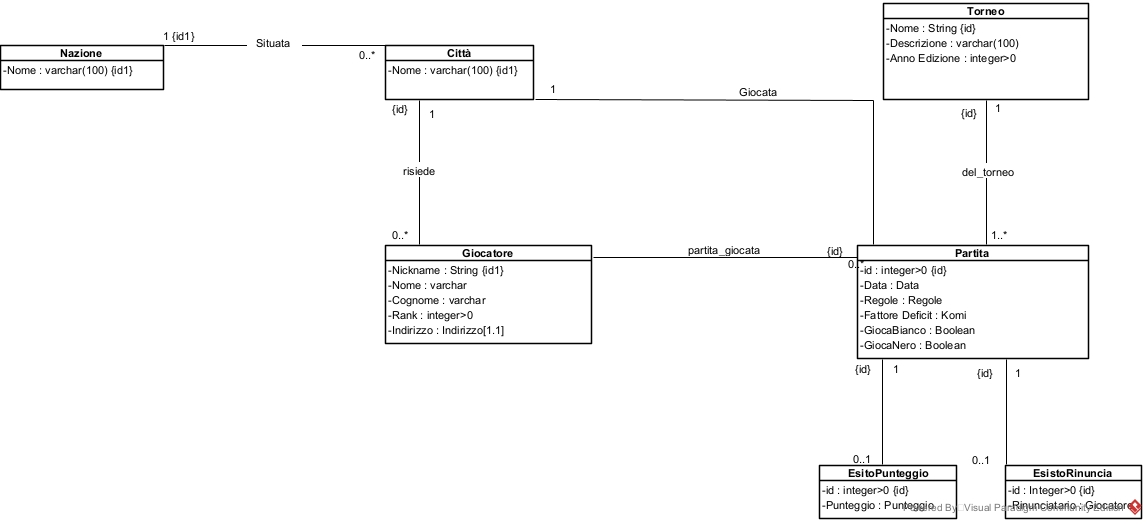
\includegraphics[width=\textwidth]{UML.jpg}
\end{center}



\end{document}

